\section{Funzione di trasferimento}

    Procediamo con il calcolo della funzione di trasferimento G(s).
    \\\\
    Avendo a disposizione le matrici A ,B ,C e D usiamo la formula:
    \begin{equation*}
        G(s)=C(sI-A)^{-1}B
    \end{equation*}
    \\
    Svolgendo i calcoli otteniamo 
    \begin{equation*}
        \resizebox*{.9\hsize}{!}{
        $G(s)=\dfrac{1}{mx_{3e}}\dfrac{s\Bigl(s+\dfrac{\beta_1}{m}\Bigr)+(k-1)\Biggl(\dfrac{2K_GM}{x^3_{3e}}+x^2_{1e}\Biggr)}
        { s\Bigl(s+\dfrac{\beta_2}{m}\Bigr)\Bigl(s+\dfrac{\beta_1}{m}\Bigr) - \dfrac{u_e}{mx_{3e}}(k-1) 
          2x_{1e}-4x^2_{1e}s(k-1)+(k-1)\Biggl(\dfrac{2K_GM}{x^3_{3e}}+x^2_{1e}\Biggr)\Bigl(s+\dfrac{\beta_2}{m}\Bigr)
        }$
        }
    \end{equation*}
    \\
    Semplificando e sostituendo i valori si ottiene:
    \begin{equation*}
        G(s)= 
        \dfrac{s^2+0.3s + 2.21\cdot 10^8}
        {3\cdot 10^7 s^3 + 1.2 \cdot 10^7 s^2 +9 \cdot 10^5 s+ 0.02}
    \end{equation*}\\
    La funzione presenta tre poli e due zeri, e presenta i seguenti diagrammi di bode

    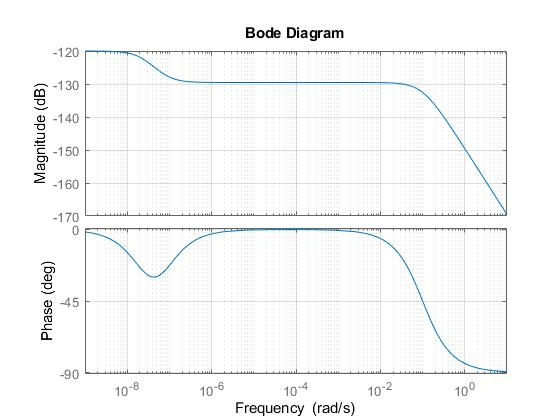
\includegraphics[scale=0.8]{./immagini/bode.jpg}
